\documentclass[red]{tutorial}
\usepackage[no-math]{fontspec}
\usepackage{xpatch}
	\renewcommand{\ttdefault}{ul9}
	\xpatchcmd{\ttfamily}{\selectfont}{\fontencoding{T1}\selectfont}{}{}
	\DeclareTextCommand{\nobreakspace}{T1}{\leavevmode\nobreak\ }
\usepackage{polyglossia} % English please
	\setdefaultlanguage[variant=us]{english}
%\usepackage[charter,cal=cmcal]{mathdesign} %different font
%\usepackage{avant}
\usepackage{microtype} % Less badboxes

%\usepackage{enumitem}

\usepackage[charter,cal=cmcal]{mathdesign} %different font
%\usepackage{euler}
 
\usepackage{blindtext}
\usepackage{calc, ifthen, xparse, xspace}
\usepackage{makeidx}
\usepackage[hidelinks, urlcolor=blue]{hyperref}   % Internal hyperlinks
\usepackage{mathtools} % replaces amsmath
\usepackage{bbm} %lower case blackboard font
\usepackage{amsthm, bm}
\usepackage{thmtools} % be able to repeat a theorem
\usepackage{thm-restate}
\usepackage{graphicx}
\usepackage{multicol}
\usepackage{fnpct} % fancy footnote spacing
\usepackage{tikz}
\usetikzlibrary{arrows.meta}
\usepackage{gensymb}

\usepackage{pgfplots}
\pgfplotsset{compat=1.18}
%\pgfkeys{/pgf/fpu}

 \usepackage{enumitem}
 
\newcommand{\xh}{{{\mathbf e}_1}}
\newcommand{\yh}{{{\mathbf e}_2}}
\newcommand{\zh}{{{\mathbf e}_3}}
\newcommand{\R}{\mathbb{R}}
\newcommand{\Z}{\mathbb{Z}}
\newcommand{\N}{\mathbb{N}}
\newcommand{\proj}{\mathrm{proj}}
\newcommand{\Proj}{\mathrm{proj}}
\newcommand{\Perp}{\mathrm{perp}}
\renewcommand{\span}{\mathrm{span}\,}
\newcommand{\Span}{\mathrm{span}\,}
\newcommand{\Img}{\mathrm{img}\,}
\newcommand{\Null}{\mathrm{null}\,}
\newcommand{\Range}{\mathrm{range}\,}
\newcommand{\rref}{\mathrm{rref}}
\newcommand{\rank}{\mathrm{rank}}
\newcommand{\Rank}{\mathrm{rank}}
\newcommand{\nnul}{\mathrm{nullity}}
\newcommand{\mat}[1]{\begin{bmatrix}#1\end{bmatrix}}
\newcommand{\chr}{\mathrm{char}}
\renewcommand{\d}{\mathrm{d}}


\theoremstyle{definition}
\newtheorem{example}{Example}[section]
\newtheorem{defn}{Definition}[section]

%\theoremstyle{theorem}
\newtheorem{thm}{Theorem}[section]

\pgfkeys{/tutorial,
	name={Tutorial 9},
	author={},
	course={MAT 187},
	date={},
	term={},
	title={Second Order Homogenous ODEs}
	}

\begin{document}
	\begin{tutorial}
		\begin{objectives}
	In this tutorial you will practise solving 2nd order homogeneous ODEs.
\end{objectives}

\vspace{-.5em}
\subsection*{Problems}
\vspace{-.5em}




%%%%%%%%%%%%%%%%%%%%%%%%%%


\begin{enumerate}
	\item Consider two differentiable, non-constant functions $y_1(t)$ and $y_2(t)$ such that:
    \begin{enumerate}[label=(\roman*)]
        \item $y_1(t) \rightarrow +\infty$ as $t \rightarrow +\infty$
        \item $y_2(t)$ is periodic.
        \item $y_2(0) = \pi$.
    \end{enumerate}

    Is it possible that both $y_1(t)$ and $y_2(t)$ solve the \textit{same} constant-coefficient ODE $ay'' + by' + cy = 0$? Explain.

    \item You're going to build a clock: an oscillator that approximately counts out short periods of time.
    You're given a spring that has damping coefficient $b=2$ kg/s and spring constant $k=2$ kg/s$^2$, and a $4$ kg mass. The corresponding ODE for this problem is given by:
    
    \[
        4y'' + 2y' + 2y = 0
    \]
    
    What is the period of the trigonometric functions found in the resulting general solution? This number is the \textbf{quasi-period}, and for small values of $b$ it approximates well the actual time between peaks of the motion. Why is this just a quasi-period and not an actual period?

    \item 
    Consider the temperature of two adjacent rooms in a house. Room $A$ has no windows, and room $B$ has windows. Denote by $A$ the temperature in room $A$ and by $B$ the temperature in room $B$. We measure temperature in degrees Celsius and time in hours.
    
    There are three effects affecting the temperature [units are given in brackets for reference]:
    \begin{itemize}[nosep,itemsep=2mm,topsep=2mm]
    	\item Effect 1: The temperature in room $A$ increases/decreases at a rate proportional to the difference in temperature between room $A$ and room $B$. The proportionality constant is $2\left[\frac{1}{h}\right]$. Note that if room $B$ is warmer than room $A$, this means that this effect warms up room $A$.
    	\item Effect 2: The temperature in room $B$ increases/decreases at a rate proportional to the difference in temperature between room $B$ and room $A$. The proportionality constant is $2\left[\frac{1}{h}\right]$. Note that if room $A$ is warmer than room $B$, this means that this effect warms up room $B$.
    	\item Effect 3: Since Room $B$ has windows, the outside temperature (day/night) affects the temperature in room $B$. This effect leads to an additional change in temperature in room $B$ of $\frac12\sin \left(\frac{\pi t}{12}\right)$ $\left[\frac{\degree C}{h}\right]$.
    \end{itemize}

\begin{enumerate}
	\item Set up an ODE describing the change in temperature in room $A$. Explain.
    \item Set up an ODE describing the change in temperature in room $B$. Explain.
    \item Manipulate the two ODEs and combine them to get an ODE that does NOT include $B$ or its derivatives. In other words, eliminate $B$ completely from the equation.
    \item Looking at the ODE you found in part (c), relate features of the ODE to the applied context. Here are some questions to consider:
	\begin{itemize}[nosep]
		\item Is this oscillator undamped, overdamped, underdamped, or criticially damped?
		\item Is this oscillator free or forced?
		\item Looking \textit{at the applied context}, why do these properties make sense?
	\end{itemize}
\end{enumerate}

\begin{minipage}{12cm}
\item The problem on the right is called a Boundary Value Problem (BVP) -- instead of an Initial Value Problem -- since there is a value given at the starting time $t=0$ and at an end time $t=t_1$.\medskip

Find a value for $t_1$ such that this BVP has a solution (there are many correct choices for $t_1$!)
\end{minipage}
\hfill
\begin{minipage}{5cm}
\[
\begin{cases}
y'' + 4y' + 5y = 0\\
y(0) = 1\\
y(t_1) = 0
\end{cases}
\]
\end{minipage}

\end{enumerate}
	\end{tutorial}

	\begin{solutions}
		

\begin{enumerate}
	\item 
    \begin{enumerate}
        \item No, this is not possible because the original ODE has units of $\frac{mass * length}{time^2}$ for each term on the left hand side, whereas the units for the terms $2y'$ and $4y$ would have different units.

        \item The characteristic equation is $r^2+2r+4 = 0$.

        \item We expect complex roots since the discriminant of the characteristic equation is negative. The roots are $-1+i\sqrt{3}$ and $-1-i\sqrt{3}$, matching our expectation.

        \item The general, complex solution to the ODE is:
        \[
        y(t) = c_1e^{(-1+i\sqrt{3})t} + c_2e^{(-1-i\sqrt{3})t}
        \]

        \item The general, real solution to the ODE is:
        \[
        y(t) = e^{-t}[c_1\cos(\sqrt{3}t)+c_2\sin{(\sqrt{3}t)}]
        \]

        \item If we graph the solution with $c_1=c_2=1$, we get the following curve:

        \begin{figure}[h]
        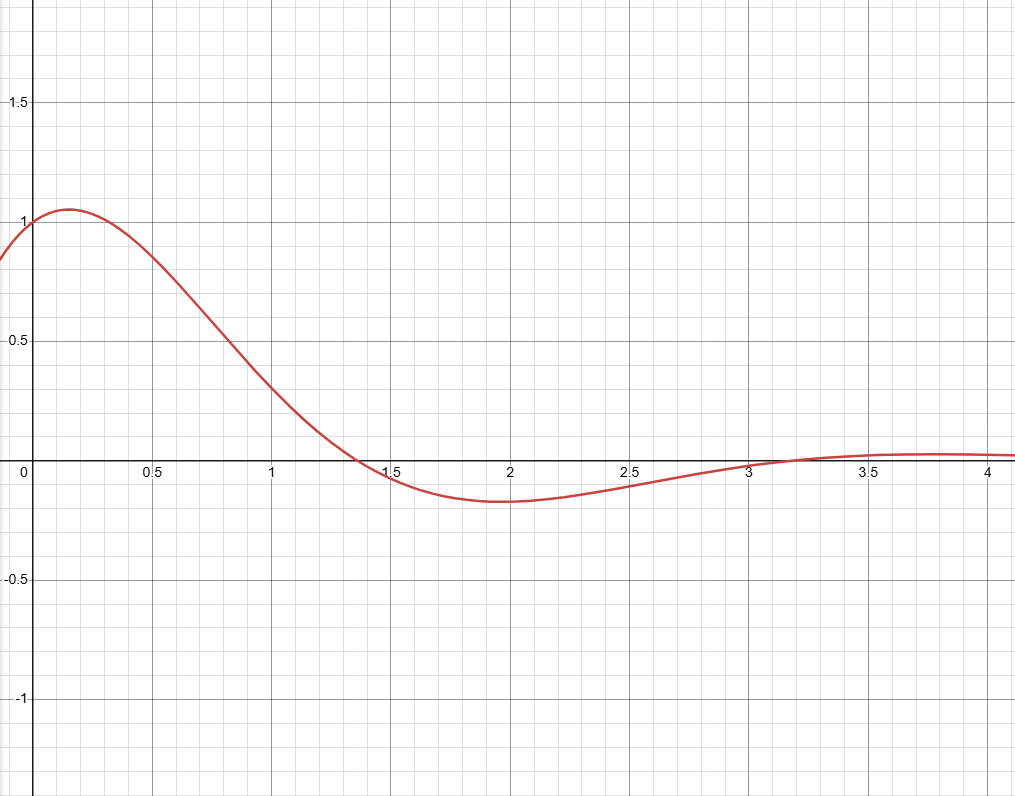
\includegraphics[width=8cm]{tutorials/Tut9_Q1.png}
        \centering
        \end{figure}

        If we were to remove the exponential factor, this would be a periodic function with a period of $\frac{2\pi}{\sqrt{3}}$ rad/s. This is what is causing the function to not be exactly periodic, so we must use the term ``quasi-periodic" instead.
    \end{enumerate}

    \item 
    \begin{enumerate}
        \item The difference between temperatures is $A - B$. Since $A'$ is proportional to this with proportionality constant 2, either $A' = 2(A- B)$ or $A' = 2(B-A)$. Since if $B > A$ means room A heats up, the second ODE is most appropriate, i.e., $A' = 2(B-A)$.

        \item Using the same argument above, we can write $B' = 2(A - B)$. However, since room B has windows, we must also add the external effect $\frac{1}{2}\sin{\frac{\pi t}{12}}$: $B' = 2(A-B) + \frac{1}{2}\sin{\frac{\pi t}{12}}$.

        \item We can derive the following:
	
    	\[
    	    A' = 2(B-A)\\
    	    \implies A'' = 2\left(B'-A'\right)\\
    	    \implies A'' = 2\left[2(A-B) + \frac{1}{2}\sin{\frac{\pi t}{12}} - A'\right]
    	\]
    	
    	Since $A' = 2(B-A)$, we can write $B = \frac{1}{2}A' + A$. Plugging this into the above yields:
    	
    	\[
    	    A'' = 2\left[2\left(A - \left(\frac{1}{2}A' + A\right)\right) + \frac{1}{2}\sin{\frac{\pi t}{12}} - A'\right]\\
    	    \implies A'' + 4A' = \sin{\frac{\pi t}{12}}
    	\]

        \item The characteristic equation is given by $r^2 + 4r = 0 \implies r_{1,2} = 0, -4$. 
	    
	    Since the roots are real, the oscillator is overdamped. Since there is a forcing function as well, the oscillator is forced. 
	    
	    In the applied context, the external forcing describes the influence of the outside temperature. The oscillator itself is a damped since, without external influence, the temperature in rooms A and B would ``balance out" over time, i.e., stabilize.
    \end{enumerate}
\end{enumerate}
	
	\end{solutions}
	\begin{instructions}
		\subsection*{Learning Objectives}
Students need to be able to\ldots
\begin{itemize}
	\item Solve 2nd order homogeneous ODEs
\end{itemize}

\subsection*{Notes}
	\begin{enumerate}
		\item 
	\end{enumerate}






	\end{instructions}

\end{document}
